%% $Id: tc.tex 52726 2016-08-04 06:31:27Z torsten $
%% $HeadURL: https://svn.cs.uni-potsdam.de/svn/reposWV/Papers/GrinGo/branches/Clingo5/tc.tex $
\documentclass[a4paper,USenglish]{oasics-v2016}

\usepackage{microtype}
\bibliographystyle{plainurl}

\usepackage[utf8]{inputenc}
\usepackage{amsmath,amssymb}
\usepackage{url}
\usepackage{wrapfig}
\usepackage{listings}
\usepackage{xcolor}
\usepackage{graphicx}

\frenchspacing
\renewcommand{\topfraction}{1}
\renewcommand{\bottomfraction}{1}

\lstset{xleftmargin=2\parindent,aboveskip=\smallskipamount,belowskip=\smallskipamount,captionpos=b}
\lstset{numbers=left,numberblanklines=false,basicstyle=\ttfamily\small}
\lstset{keywords=[1]{m,n},keywordstyle=[1]\usefont{OT1}{cmtt}{m}{n}}

\lstdefinelanguage{clingo}{
  keywordstyle=[1]\usefont{OT1}{cmtt}{m}{n},%
  keywordstyle=[2]\textbf,%
  keywordstyle=[3]\usefont{OT1}{cmtt}{m}{n},%\textit
  alsoletter={\#,\&},%
  keywords=[1]{not,from,import,def,if,else,return,while,break,and,or,for,in,del,and,class},%
  keywords=[2]{\#const,\#show,\#minimize,\#base,\#theory,\#count,\#external,\#program,\#script,\#end,\#heuristic,\#edge,\#project,\#show},%
  keywords=[3]{&,&dom,&sum,&diff,&show},%
  morecomment=[l]{\#\ },%
  morecomment=[l]{\%\ },%
  commentstyle={\color{darkgray}}%
}

\newcommand{\gringo}{\textit{gringo}}
\newcommand{\clasp}{\textit{clasp}}
\newcommand{\clingo}{\textit{clingo}}
\newcommand{\asprin}{\textit{asprin}}
\newcommand{\asap}{\textit{teaspoon}}
\newcommand{\piclasp}{\textit{piclasp}}

\newcommand{\code}[1]{\lstinline[basicstyle=\ttfamily]{#1}}

\newcommand{\lw}[1]{\smash{\lower1.ex\hbox{#1}}}
\newcommand{\llw}[1]{\smash{\lower3.ex\hbox{#1}}}

%\newcommand{\dataCL}[5]{%
%  \code{#1} & #3 & #5 & #4
%}
%\newcommand{\dataCS}[5]{%
%  #3 & #5 & #4
%}

\newenvironment{tableC}{%
  \scriptsize
  \tabcolsep = 0.6mm
  \begin{tabular}[t]{l|rlr|rlr|rlr|rlr|rlr}\hline
    \multicolumn{1}{l|}{\llw{Instance}} &
    \multicolumn{3}{c|}{UD1} &
    \multicolumn{3}{c|}{UD2} &
    \multicolumn{3}{c|}{UD3} &
    \multicolumn{3}{c|}{UD4} &
    \multicolumn{3}{c}{UD5} \\
    & 
    \multicolumn{1}{c}{Best} & & \multicolumn{1}{c|}{\emph{tea-}} & 
    \multicolumn{1}{c}{Best} & & \multicolumn{1}{c|}{\emph{tea-}} & 
    \multicolumn{1}{c}{Best} & & \multicolumn{1}{c|}{\emph{tea-}} & 
    \multicolumn{1}{c}{Best} & & \multicolumn{1}{c|}{\emph{tea-}} & 
    \multicolumn{1}{c}{Best} & & \multicolumn{1}{c}{\emph{tea-}} \\
    & 
    known & & \emph{spoon} & 
    known & & \emph{spoon} & 
    known & & \emph{spoon} & 
    known & & \emph{spoon} & 
    known & & \emph{spoon} \\
    \hline
  }{%
    \hline
  \end{tabular}
}

\newenvironment{tableB}{%
  \scriptsize
  \tabcolsep = 0.7mm
%  \begin{tabular}[t]{|l|c|r|l|l|l|}\hline
  \begin{tabular}[t]{lcrlll}\hline
    Instance &
    Formulation &
    Time (sec.)\\
    \hline
  }{%
    \hline
  \end{tabular}
}
\newenvironment{tableL}{%
  \scriptsize
  \tabcolsep = 0.7mm
  \begin{tabular}[t]{l|rrrrrrrr|r}\hline
    \lw{Instance} &
    \lw{Time (sec.)} &
    \multicolumn{6}{c}{The best utility vector} &
    The sum of  &
    The best of basic\\
    &
    &
    $(S_1,$ & $S_4,$ & $S_2,$ & $S_7,$ & $S_6,$ & $S_3)$ &
    utility vector &
    and optimized \\
    \hline
  }{%
    \hline
  \end{tabular}
}

%%% Local Variables:
%%% mode: latex
%%% TeX-master: "paper"
%%% End:


\title{Theory Solving Made Easy with \textit{Clingo}~5\footnote{This work was partially supported by DFG-SCHA-550/9}}
\titlerunning{Theory Solving Made Easy with \textit{Clingo}~5}

\author[1]{Martin~Gebser}
\author[1]{Roland~Kaminski}
\author[1]{Benjamin~Kaufmann}
\author[1]{Max~Ostrowski}
\author[1,2]{Torsten~Schaub}
\author[1]{Philipp~Wanko}

\affil[1]{University of Potsdam, Germany}
\affil[2]{INRIA Rennes, France}

\authorrunning{M. Gebser, R. Kaminski, B. Kaufmann, M. Ostrowski, T. Schaub, and P. Wanko}

\Copyright{M. Gebser, R. Kaminski, B. Kaufmann, M. Ostrowski, T. Schaub, and P. Wanko}%mandatory, please use full first names. OASIcs license is "CC-BY";  http://creativecommons.org/licenses/by/3.0/

\subjclass{D.1.6 Logic Programming}
\keywords{Answer Set Programming, Theory Language, Theory Propagation}

\pdfinfo{
/Title (Theory Solving Made Easy with Clingo 5)
/Author (Martin~Gebser, Roland~Kaminski, Benjamin~Kaufmann, Max~Ostrowski, Torsten~Schaub, Philipp~Wanko) }

%%%%%%%%%%%%%%%%%%%%%%%%%%%%%%%%%% 
%Editor-only macros:: begin
\EventEditors{Manuel Carro, Andy King, Marina De Vos, and Neda Saeedloei}
\EventNoEds{4}
\EventLongTitle{Technical Communications of the 32nd Int'l Conference on Logic
      Programming (ICLP 2016)}
\EventShortTitle{ICLP 2016 TCs}
\EventAcronym{ICLP}
\EventYear{2016}
\EventDate{October 16--21, 2016}
\EventLocation{New York City, USA}
\EventLogo{}
\SeriesVolume{52}
\ArticleNo{NNN}
% Editor-only macros::end %%%%%%%%%%%%%%%%%%%%%%%%%%%%%%%%%%%%%%%%%%%%%%%

\begin{document}

\maketitle

%\begin{abstract}
%	The design space for highly complex system level specifications of embedded systems is enormous as tasks may be mapped to different resources and messages may be routed over several links of the hardware platform. 
%	Furthermore, highly constrained requirements lead to many infeasible solutions that have to be sorted out. \emph{\ac{ASP}} in combination with variant background theories (\emph{\ac{ASPmT}}) has been shown to cope with such requirements very efficiently. However, especially in system level design, a fast \emph{\ac{DSE}} including optimization is crucial in order to steer the development towards optimal design points. In this paper, we therefore propose to couple the highly efficient constraint solving capabilities of \ac{ASP} with a \ac{DSE} including \emph{multi-objective optimization} in an additional background theory. Utilizing the possibility to work on \emph{partial assignments}, \ac{ASPmT} is able to prune entire infeasible and dominated regions from the search space early in the decision process. In the experimental section, we present and compare variant approaches and domain specific heuristics.
%\end{abstract}

\begin{abstract}
	An efficient \emph{\ac{DSE}} is imperative for the design of modern, highly complex embedded systems in order to steer the development towards optimal design points. The early evaluation of design decisions at system-level abstraction layer helps to find promising regions for subsequent development steps in lower abstraction levels by diminishing the complexity of the search problem. In recent works, symbolic techniques, especially \ac{ASPmT}, have been shown to find feasible solutions of highly complex system-level synthesis problems with non-linear constraints very efficiently. In this paper, we present a novel approach to a holistic system-level \ac{DSE} based on \ac{ASPmT}. To this end, we include additional background theories that concurrently guarantee compliance with hard constraints and perform the simultaneous optimization of several design objectives. %First experimental results show the applicability of our approach. %for large optimization of up to 170 tasks mapped to 3-dimensional hardware platforms. Furthermore, it outperforms current multi-objective optimization strategies of \ac{ASP} with respect to both diversity and convergence of found solutions.   %We present and investigate several strategies that show the applicability of our approach even for large problem instances. 
	We implement and compare our approach with a state-of-the-art preference handling framework for \ac{ASP}. Experimental results indicate that our proposed method produces better solutions with respect to both diversity and convergence to the true Pareto front.
\end{abstract}

\section{Introduction}
\label{sec:introduction}
%In order to cope with the ever-increasing complexity of embedded systems, system level description are utilized to diminish the complexity of finding potentially good solutions which can then be used as initial starting points for further optimization in lower abstraction levels. On system level, applications are composed of granular tasks that exchange information over communication messages and form dependency relations between each other. The hardware architecture contains heterogeneous processing elements (e.g.~CPU, DSP, GPU) as well as a communication infrastructure like routers and links. Yet, the design space for such system level specifications of embedded systems is still enormous as tasks may be mapped to different computational resources and messages may be routed over several links of the communication infrastructure.\par 
%Furthermore, various hard constraints like maximum latency and energy consumption of the resulting systems have to be considered. That is, only a subset of all possible decisions leads to valid system implementations that conform to previously defined constraints which makes it even hard\footnote{In fact, the mapping problem is known to be $\mathcal{NP}$-hard \cite{Blickle1998}.} to find \emph{one} feasible solution. However, by encoding the problem symbolically (cf.~\cite{Haubelt2003}) and due to the technological advances in \ac{SAT}, various constraint solvers can be utilized to cope with the complexity. Especially, \emph{\acf{ASP}} has been shown to deal with such stringently constrained design problems very efficiently (e.g.~\cite{Andres2013}). Opposed to other symbolic techniques like \ac{SAT}, reachability can be expressed naturally in \ac{ASP} which fastens the routing sub-problem.\par 
%%\ac{ASP} stems from the area of knowledge representation and reasoning and is based on the \emph{stable model semantics}. 
%Finding one feasible solution is however often insufficient. Depending on the decisions that have been made, the qualitative properties (e.g.~latency, energy consumption, area requirements) of the resulting system implementation may vary considerably from solution to solution. Thus, a \acf{DSE} is imperative to find solutions with optimal properties. Usually, the objectives (i.e.~optimizing the individual properties) of \acp{MOOP} are conflicting with each other and no single optimal solution but a set of \emph{Pareto optimal} solutions exists. A Pareto optimal solution is characterized by the property that it is not dominated by (i.e.~not worse in all objectives than) any other solution. \par%That is, all Pareto optimal solutions are mutually non-dominated.\par 
%Commonly, meta-heuristics like \acp{MOEA} are utilized to solve \acp{MOOP}. They are based on natural processes and work on sets of solutions (populations) concurrently. Each solution is evaluated by a fitness function with respect to the objectives and the best solutions are combined to create novel solutions for subsequent generations. As the initial population is created by a randomized process, finding feasible solutions becomes a problem for stringently constraint environments. Moreover, because the search is generally not executed systematically but based on combining previously found solutions, \acp{MOEA} tend to run into saturation and stop finding novel solutions after an arbitrary number of iterations.\par
%In the paper at hand, we therefore propose an approach that utilizes an exact symbolic encoding for both the constraint solving and the design space exploration. Based on \ac{ASP}, we tightly integrate background theory solvers, known as \ac{ASPmT}, that handle (non-)linear objectives as well as Pareto filtering of found solutions. Furthermore, they are able to work on partial solutions to prune the search space from infeasible and dominated regions of design points early in the decision process. 
%The contribution of this paper is threefold:
%\begin{enumerate}
%	\item We present a universal framework for preference handling that is capable of both linear and non-linear objectives based on \ac{ASPmT}.
%	\item In order to combine various background theories for multi-objective optimization and constraint solving concurrently, we present various approaches.
%	\item Extensive experimental test instances show the advantages and disadvantages of the different approaches. 
%\end{enumerate}\par
%\textbf{Paper organization:} Related work will be covered in Sec.~\ref{sec:relatedwork}. Afterwards, the execution model that will be used throughout the paper is briefly described in Sec.~\ref{sec:model}. Section \ref{sec:framework} contains detailed information about our proposed preference handling framework. Experimental results are given in Sec.~\ref{sec:experiments} before Sec.~\ref{sec:conclusion} concludes the paper.

%Essentially, there are three approaches to explore the design space \cite{Pimentel2017}: First, meta-heuristics like evolutionary algorithms have been studied thoroughly in the past (e.g.~\cite{1,2,3,4,5}). Those techniques are inspired by the natural selection process and work on whole sets of solutions (populations) concurrently. Each solution is evaluated and the best are combined to create new solutions for the following generations. One major problem arises if, due to various hard constraints, only a small subset of design points is feasible. Because of their random nature, pure meta-heuristics tend to fail in finding feasible regions of the design space. \par 
%Therefore, the second approach type combines meta-heuristics with exact methods (e.g.~\cite{Neubauer2016,Haubelt2003,Lukasiewycz2012a}). That is, not the decision variables themselves but the heuristics that are used by the constraint solver are subject to the randomized exploration process. Every found design point is thereby guaranteed to be feasible.\par 
%Finally, exact methods have been developed to explore the design space systematically. While meta-heuristics normally only cover a limited portion of the design space, exact methods (e.g.~\cite{6,7,8,9}) such as \ac{ILP} and branch-and-bound algorithms are guaranteed to find the optimal solutions. \par
%However, the latter are often infeasible for real-world problems as the design space is simply too vast to evaluate every design point.
%However, finding even \emph{one} feasible solution that conforms to all constraints is an $\mathcal{NP}$-hard problem (cf.~\cite{Blickle1998}).
%One way to cope with such complexities is to represent such problems symbolically and utilize specialized solvers like \ac{SAT} (e.g.~\cite{Neubauer2016}), \ac{ILP} (e.g.~\cite{Lukasiewycz2008}), or \acf{ASP} (e.g.~\cite{Andres2013}). 
%In combination with variant background theories, known as \acf{ASPmT}, it is able to handle non-linear constraints like latency and energy calculations (\cite{Andres2015,Neubauer2017}). Bases on \ac{ASP}, the preference handling framework  that is able to compute preferred (optimal) solutions.

%\begin{itemize}
%	\item Partial solutions $\ldots$ dominance checks, infeasibility
%	\item MOEAs three problems: saturation, finding initial solutions, complete solutions
%	\item symbolic encoding
%\end{itemize}>>>>>>> .r56897


In order to cope with the ever-increasing complexity of embedded systems, system-level descriptions are utilized to diminish the complexity of finding potentially good solutions which can then be used as initial starting points for further optimization in lower abstraction levels. At system level, applications are composed of communicating tasks while the hardware architecture contains heterogeneous processing elements (e.g.~CPU, DSP, GPU) as well as a communication infrastructure like routers and links. 
%Yet, the design space for such system-level specifications of embedded systems is still enormous as tasks may be mapped to different computational resources and communication messages may be routed over several links of the communication infrastructure.\par 
%Furthermore, various hard constraints like maximum latency and energy consumption of the resulting systems have to be considered. That is, only a subset of all possible decisions leads to valid system implementations that conform to previously defined constraints which makes it even hard\footnote{In fact, the mapping problem is known to be $\mathcal{NP}$-hard \cite{Blickle1998}.} to find \emph{one} feasible solution. However, by encoding the problem symbolically (cf.~\cite{Haubelt2003}) and due to the technological advances in \ac{SAT}, various constraint solvers can be utilized to cope with the complexity. Especially, \emph{\acf{ASP}} has been shown to deal with such stringently constrained design problems very efficiently (e.g.~\cite{Andres2013}). Opposed to other symbolic techniques like \ac{SAT}, reachability can be expressed naturally in \ac{ASP} which fastens the routing sub-problem.\par 
%\ac{ASP} stems from the area of knowledge representation and reasoning and is based on the \emph{stable model semantics}. 
%Finding one feasible solution is however often insufficient. Depending on the decisions that have been made, the qualitative properties (e.g.~latency, energy consumption, area requirements) of the resulting system implementation may vary considerably from solution to solution. Thus, a \acf{DSE} is imperative to find solutions with optimal properties. Usually, the objectives (i.e.~optimizing the individual properties) of \acp{MOOP} are conflicting with each other and no single optimal solution but a set of \emph{Pareto optimal} solutions exists. A Pareto optimal solution is characterized by the property that it is not dominated by (i.e.~not worse in all objectives than) any other solution. \par%That is, all Pareto optimal solutions are mutually non-dominated.\par 

Depending on the decisions that have been made, the qualitative properties (e.g.~latency, energy consumption, area requirements) of the resulting system implementation may vary considerably from solution to solution resulting into a \ac{MOOP}. Thus, a \acf{DSE} is imperative to find solutions with optimal properties. \par
Essentially, \ac{DSE} approaches can be characterized into two types \cite{Pimentel2017}: First, (meta-)heuristics like evolutionary algorithms and ant colony optimization (e.g.~\cite{Thompson2013,Ferrandi2010}) and second, exact methods such as \ac{ILP} and branch-and-bound algorithms (e.g.~\cite{Lukasiewycz2008,Khalilzad2016}). \par 
Most of the works presented in the field of meta-heuristics extend basic techniques in order to respect domain specific characteristics. For example, in \cite{Thompson2013}, the authors extend genetic algorithms by utilizing domain knowledge. They state, that small differences in design decisions lead to similar system implementations and that symmetrical design points can be pruned. \par 
Another approach (e.g. \cite{Neubauer2016,Schlichter2006}) of handling the infeasibility problem is to integrate dedicated constraint solvers into a \ac{MOEA}. The work of Schlichter et al. \cite{Schlichter2006} integrates, for example, a \ac{SAT} solver into a \ac{MOEA}. Here, the decisions are not directly controlled by the randomized search algorithm of the \ac{MOEA} but the heuristic of the decision variables is subject to exploration. This way, solutions are guaranteed to be feasible.\par
Finally, fully exact methods have been developed to explore the design space systematically. While meta-heuristics normally only cover a limited portion of the design space, exact methods are guaranteed to find the optimal solutions. Nevertheless, for a long time those methods were restricted to single-objective optimization problems only. As one of the few exceptions, Lukasiewycz et al.  \cite{Lukasiewycz2008} present a complete multi-objective Pseudo-Boolean solver based on branch-and-bound algorithms. The results show that this technique is able to find the proven optimal solutions for small problems in a short time. However, exact methods are often replaced in favor of heuristic approaches as the complexity of large systems hinders reasonable employment of those techniques. \par
The disadvantage of using meta-heuristics, on the other hand, is that the initial population is created by a randomized process. Finding feasible regions becomes therefore a problem for stringently constraint environments. Moreover, because the search is generally not executed systematically but based on combining previously found solutions, \acp{MOEA} tend to run into saturation and stop finding novel solutions after a number of iterations.\par
As a remedy, by encoding the problem symbolically, recent advances of constraint solving technologies can be utilized to cope with the complexity of finding feasible solutions. Especially, \emph{\acf{ASP}} has been shown to deal with such stringently constrained design problems very efficiently (e.g.~\cite{Andres2013}). Opposed to other symbolic techniques like \ac{SAT}, reachability can be expressed naturally in \ac{ASP} which fastens the communication synthesis. However, one problem is that non-linear constraints cannot be easily expressed within \ac{ASP}. \par
In the paper at hand, we therefore propose an approach that utilizes an exact symbolic encoding for both constraint solving and design space exploration. To address the shortcomings of \ac{ASP}, we present specific background theory solvers to handle \emph{non-linear objectives} as well as Pareto filtering of found solutions. By utilizing the state-of-the-art \ac{ASP} solver clingo~5 \cite{gekakaosscwa16a}, these background theories can be tightly integrated into the solving process (\emph{\acf{ASPmT}}). This way, we are able to utilize conflict clauses on partial solutions to prune the search space from infeasible and dominated regions of design points early in the decision process. \par
Note that our methodology uses \emph{exact} search strategies with "\emph{any-time}" characteristic, i.e., canceling the search at any time returns an approximate Pareto set that strictly improves with increased solving time until the true Pareto front is reached.\par
%\textbf{Paper organization and contribution:} In the following, we will first reflect upon related work in Sec.~\ref{sec:relatedwork} before the considered specification model and the basics of \ac{ASPmT} are presented in Sec.~\ref{sec:model}. Section \ref{sec:framework} contains the main contribution of the work at hand. Here, we present our proposed universal framework for \acf{DSE} that is capable of multi-objective optimization of both linear and non-linear objectives. For the first time, various approaches for handling the Pareto filtering in a background theory will be presented.    Afterwards, in Sec.~\ref{sec:experiments}, the approaches are evaluated by a number of differently configured test instances. Finally, Sec.~\ref{sec:conclusion} concludes the paper.

%The contribution of this paper is threefold:
%\begin{enumerate}
%	\item We present a universal framework for preference handling that is capable of both linear and non-linear objectives based on \ac{ASPmT}.
%	\item In order to combine various background theories for multi-objective optimization and constraint solving concurrently, we present various approaches.
%	\item Extensive experimental test instances show the advantages and disadvantages of the different approaches. 
%\end{enumerate}\par
%\textbf{Paper organization:} Related work will be covered in Sec.~\ref{sec:relatedwork}. Afterwards, the execution model that will be used throughout the paper is briefly described in Sec.~\ref{sec:model}. Section \ref{sec:framework} contains detailed information about our proposed preference handling framework. Experimental results are given in Sec.~\ref{sec:experiments} before Sec.~\ref{sec:conclusion} concludes the paper.

\section{Input Language}\label{sec:language}

This section introduces the novel features of \clingo~5's input language.
All of them are situated in the underlying grounder \gringo~5 and can thus
also be used independently of \clingo.
%
We start with a detailed description of \gringo~5's generic means for defining theories
and afterwards summarize further % the remaining 
new features.

Our generic approach to theory specification rests upon two languages:
the one defining theory languages and the theory language itself.
Both borrow elements from the underlying ASP language,
foremost an aggregate-like syntax for formulating variable length expressions.
To illustrate this, consider Listing~\ref{prg:diff},
where a logic program is extended by constructs for handling difference and linear constraints.
While the former are binary constraints of the form $x_1-x_2\leq k$, % where $x,y$ are integer variables and $k$ is an integer,
the latter have a variable size and are of form
\(
a_1x_1+\dots+a_nx_n\circ k
\),
where $x_i$ are integer variables, $a_i$ and $k$ are integers, and $\circ\in\{\leq,\geq,<,>,=\}$
for $1\leq i\leq n$.%
\footnote{For simplicity, we consider normalized difference constraints rather than general ones of form $x_1-x_2\circ k$.}
Note that solving difference constraints is polynomial, while solving linear equations (over integers) is NP-hard.
The theory language for expressing both types of constraints is defined in Lines~\ref{prg:diff:begin-theory}--\ref{prg:diff:end-theory} and preceded by the directive \lstinline{#theory}.
The elements of the resulting theory language are preceded by \lstinline{&} and used as regular atoms in the logic program in Lines~\ref{prg:diff:begin-program}--\ref{prg:diff:end-program}.
% ------------------------------------------------------------
\lstinputlisting[language=clingo,morekeywords={n,m},float=t,escapeinside={\%(}{\%)},basicstyle=\ttfamily\small,label=prg:diff,caption=Logic program enhanced with difference and linear constraints (\texttt{diff.lp})]{code/diff.lp}
% ------------------------------------------------------------

To be more precise,
a \emph{theory definition} has the form
\begin{lstlisting}[numbers=none,mathescape=t]
#theory $T$ {$D_1$;$\dots$;$D_n$}.
\end{lstlisting}
where $T$ is the theory name and each $D_i$ is a definition for a theory term or a theory atom for $1\leq i\leq n$.
The language induced by a theory definition is the set of all theory atoms constructible from its theory atom definitions.

A \emph{theory atom definition} has form
\begin{lstlisting}[numbers=none,mathescape=t]
&$p$/$k$ : $t$,$o$ $\quad\textrm{ or }\quad$ &$p$/$k$ : $t$,{$\diamond_1$,$\dots$,$\diamond_m$},$t'$,$o$
\end{lstlisting}
where $p$ is a predicate name and $k$ its arity,
$t,t'$ are names of theory term definitions,
each $\diamond_i$ is a theory operator for $m\geq 1$,
and
\(
o\in\{\mathtt{head},\mathtt{body},\mathtt{any}, \mathtt{directive}\}
\)
determines where theory atoms may occur in a rule.
%
Examples of theory atom definitions are given in Lines~\ref{lst:ex1-begin-def-atom}--\ref{lst:ex1-end-def-atom} of Listing~\ref{prg:diff}.
%%
The language of a theory atom definition as above contains all \emph{theory atoms} of form
\begin{lstlisting}[numbers=none,mathescape=t]
&$a$ {${C}_1$:${L}_1$;$\dots$;${C}_n$:${L}_n$}$\quad\textrm{ or }\quad$ &$a$ {${C}_1$:${L}_1$;$\dots$;${C}_n$:${L}_n$} $\diamond$ $c$
\end{lstlisting}
where $a$ is an atom over predicate $p$ of arity $k$,
each ${C}_i$ is a tuple of theory terms in the language for~$t$,
$c$ is a theory term in the language for~$t'$,
$\diamond$ is a theory operator among $\{ \diamond_1, \dots, \diamond_m \}$,
and each ${L}_i$ is a regular condition (i.e., a tuple of regular literals)
for $1\leq i\leq n$.
% The last part `${}\diamond c$' is optional.
Whether the last part `${}\diamond c$' is included depends on the form of a theory atom definition.
%
Five occurrences of theory atoms can be found in Lines~\ref{prg:diff:begin-use-theory}--\ref{prg:diff:end-use-theory} of Listing~\ref{prg:diff}.

A \emph{theory term definition} has form
\begin{lstlisting}[numbers=none,mathescape=t]
$t$ {$D_1$;$\dots$;$D_n$}
\end{lstlisting}
where $t$ is a name for the defined terms and each $D_i$ is a theory operator definition 
for $1\leq i\leq n$.
A respective definition specifies the language of all theory terms
that can be constructed via % admissible term constructors and
its operators. % , as described next.
%
Examples of theory term definitions are given in Lines~\ref{prg:diff:begin-def-term}--\ref{prg:diff:end-def-term} of Listing~\ref{prg:diff}.
%%
Each resulting \emph{theory term} is one of the following:
\par\medskip\noindent
\begin{minipage}{0.5\linewidth}
  \begin{itemize}
  \item a constant term: \ $c$
  \item a variable term: \ $v$
  \item a binary theory term: \  $t_1 \diamond t_2$
  \item a unary theory term: \  ${}\diamond t_1$
  \end{itemize}
\end{minipage}
\begin{minipage}{0.5\linewidth}
\begin{itemize}
  \item a function theory term: \  $f(t_1,\dots,t_k)$
  \item a tuple theory term: \  $(t_1,\dots,t_l,)$
  \item a set theory term: \  $\{t_1,\dots,t_l\}$
  \item a list theory term: \  $[t_1,\dots,t_l]$
\end{itemize}
\end{minipage}
\par\medskip\noindent
where each $t_i$ is a theory term,
$\diamond$ is a theory operator defined by some $D_i$,
$c$ and $f$ are symbolic constants,
$v$ is a first-order variable,
$k\geq 1$, and
$l\geq 0$.
(The trailing comma in tuple theory terms is optional if $l \neq 1$.)
% Furthermore,
Parentheses can be used to specify operator precedence.

A \emph{theory operator definition} has form
\begin{lstlisting}[numbers=none,mathescape=t]
$\diamond$ : $p$,unary $\quad\textrm{ or }\quad$ $\diamond$ : $p$,binary,$a$
\end{lstlisting}
where $\diamond$ is a unary or binary theory operator with precedence $p\geq 0$
(determining implicit parentheses). % , respectively.
Binary theory operators are additionally characterized by an associativity
$a\in\{\text{\lstinline{right}},\linebreak[1]\text{\lstinline{left}}\}$.
%
As an example,
consider Line~\ref{prg:diff:op-mul} of Listing~\ref{prg:diff},
where the \lstinline{binary} operator~\lstinline{*} is defined with precedence~\lstinline{1} and \lstinline{left} associativity.
%
In total, Lines~\ref{prg:diff:begin-def-term}--\ref{prg:diff:end-def-term} of Listing~\ref{prg:diff}
include nine theory operator definitions.
%%
Particular \emph{theory operators} can be assembled (written consecutively without spaces) from the symbols
`\lstinline{!}',
`\lstinline{<}',
`\lstinline{=}',
`\lstinline{>}',
`\lstinline{+}',
`\lstinline{-}',
`\lstinline{*}',
`\lstinline{/}',
`\lstinline{\}',
`\lstinline{?}',
`\lstinline{&}',
%`\texttt{\&}',
`\lstinline{|}',
`\lstinline{.}',
`\lstinline{:}',
`\lstinline{;}',
`\lstinline{~}', and
`\lstinline{^}'.
%
For instance,
in Line~\ref{prg:diff:op-dot} of Listing~\ref{prg:diff}, the operator `\lstinline{..}' is defined as the concatenation of two periods.
%
% Note that
The tokens
`\lstinline{.}',
`\lstinline{:}',
`\lstinline{;}', and
`\lstinline{:-}'
must be combined with other symbols
due to their dedicated usage.
Instead, one may write
`\lstinline{..}',
`\lstinline{::}',
`\lstinline{;;}',
`\lstinline{::-}',
etc.
% Each operator is either unary or binary.
% To resolve ambiguities,
% a binary theory operator is either left or right associative.
% Furthermore, each operator has a precedence to allow for omitting parentheses in some situations.

While theory terms are formed similar to regular ones,
theory atoms rely upon an aggregate-like construction for forming variable-length theory expressions.
In this way, standard grounding techniques can be used for gathering theory terms.
(However, the actual atom within a theory atom comprises regular terms only.)
%
The treatment of theory terms still % and atoms % is different
differs from their regular counterparts
% This is due to the fact 
in that the grounder skips simplifications like, e.g., arithmetic evaluation.
% completely ignores the theory's semantics and thus performs no theory-specific simplifications.
This can be nicely seen on the different results in Listing~\ref{prg:grd:diff} of grounding terms formed with
the regular and theory-specific variants of operator `\lstinline{..}'.
Observe that
the     fact \lstinline{task(1..n)} in Line~\ref{prg:diff:rule-task} of Listing~\ref{prg:diff} results in \lstinline{n} ground     facts,
viz.\ \lstinline{task(1)} and \lstinline{task(2)} because of \lstinline{n=2}.
Unlike this, the theory expression \lstinline{1..m} stays structurally intact and is only transformed into \lstinline{1..1000} in view of \lstinline{m=1000}.
That is, the grounder does not evaluate the theory term \lstinline{1..1000} and
leaves its interpretation to a downstream theory solver.
%
% ------------------------------------------------------------
\lstinputlisting[language=clingo,float=t,basicstyle=\ttfamily\small,label=prg:grd:diff,caption={Human-readable result of grounding Listing~\ref{prg:diff} via `\texttt{gringo --text diff.lp}'}]{code/diff.grd}
% ------------------------------------------------------------
%
A similar situation is encountered when comparing the treatment of the regular term `\lstinline{200*T}' in Line~\ref{prg:diff:rule-duration} of Listing~\ref{prg:diff} to the
theory term `\lstinline{end(T)-start(T)}' in Line~\ref{prg:diff:rule-diff}.
While each instance of `\lstinline{200*T}' is evaluated during grounding,
instances of the theory term  are left in Line~6 of Listing~\ref{prg:grd:diff}.
In fact, if `\lstinline{200*T}' had been a theory term as well,
it would have resulted in the unevaluated instances  `\lstinline{200*1}' and `\lstinline{200*2}'. % , respectively.
% This is because the grounder ignores the meaning of the theory operator `\lstinline{*}'.

The remainder of this section is dedicated to other language extensions of \gringo~5 aiming
at a disentanglement of the various uses of \lstinline{#show} directives
(and their induced symbol table).
Such directives were beforehand used for
controlling the output of stable models,
delineating the scope of reasoning modes (e.g., intersection, union, projection, etc.),
and for
passing special-purpose information to downstream systems.
For instance,
theory and heuristic information was passed to \clasp\ via dedicated predicates like \lstinline{_edge} and \lstinline{_heuristic}.
This entanglement brought about several shortcomings.
% For one, the output of reasoning modes had to coincide with the atoms subject to the reasoning mode.
In fact, passing information via a symbol table did not only scramble the output, but also provoked overhead in grounding and filtering ``artificial'' symbolic information.

Now, in \gringo~5, the sole purpose of \lstinline{#show} is to furnish an output directive.
There are three different kinds of such statements:
%
\begin{lstlisting}[numbers=none,mathescape=t]
#show.     #show $p$/$n$.      #show $t$ : $l_1$,$\dots$,$l_n$.
\end{lstlisting}
%
The first form hides all atoms, and the second all except those over predicates~$p/n$ indicated by \lstinline{#show} statements.
The third form does not hide any atoms and can be used to output arbitrary terms~$t$,
whenever the literals $l_1,\dots,l_n$ in the condition after~`\lstinline{:}' hold.
This is particularly useful in meta-programming,
e.g., `\lstinline{#show A : holds(A).}' can be used to map back reified atoms.

Atoms used in reasoning modes are indicated by \lstinline{#project} directives, having two forms:
%
\begin{lstlisting}[numbers=none,mathescape=t]
#project $p$/$n$.     #project $a$ : $l_1$,$\dots$,$l_n$.
\end{lstlisting}
%
Here, $p$ is a predicate name with arity $n$, $a$ is an atom, and $l_1,\dots,l_n$ are % regular
literals.
While the first form declares all atoms over predicate~$p/n$ as % being
subject to projection,
the second includes instances of~$a$
obtained via grounding, as detailed in \cite{gekakasc14b} for
\lstinline{#external} directives.

The last two new directives of interest abolish the need for % using
the special-purpose predicates \lstinline{_edge} and \lstinline{_heuristic},
previously used in conjunction with the ASP solver \clasp:
\begin{lstlisting}[numbers=none,mathescape=t]
#edge ($u$,$v$) : $l_1$,$\dots$,$l_n$.
#heuristic $a$ : $l_1$,$\dots$,$l_n$. [$k$@$p$,$m$]
\end{lstlisting}
As above, $a$ is an atom, and $l_1,\dots,l_n$ are literals.
Moreover,
$u,v,k,p,m$ are terms, % is a condition;
where 
`\lstinline[mathescape=t]{($u$,$v$)}' stands for an
edge from $u$ to $v$ in an acyclicity extension \cite{bogejakasc15a}.
Integer values for $k$ and $p$ along with
\lstinline{init}, \lstinline{factor}, \lstinline{level}, \lstinline{sign}, \lstinline{true}, or \lstinline{false} for~$m$
determine a heuristic modifier \cite{gekaotroscwa13a}.
Finally, note that
zero is taken as default priority when
the optional `\lstinline[mathescape=t]{@$p$}' part 
in `\lstinline[mathescape=t]{[$k$@$p$,$m$]}',
resembling the syntax of ranks for weak constraints \cite{aspcore2},
is omitted.
% $k$ is a term evaluating to an integer and $m$ is a heuristic modifier among
% \lstinline{init}, \lstinline{factor}, \lstinline{level}, \lstinline{sign}, \lstinline{true}, or \lstinline{false}, respectively.
% A positive integer priority $p$ is optional (and zero by default).
% Note that the usage of the term \lstinline[mathescape=t]{[$k$@$p$,$m$]} is borrowed from weak constraints~\cite{aspcore2}.
% Also, observe that arcs \lstinline[mathescape=t]{($u$,$v$)} and heuristically modified atoms $a$ can still be defined (recursively) via arbitrary subprograms,
% but now without any need to show them in a resulting stable models.
% %
% We refer the reader to \cite{bogejakasc15a} and \cite{gekaotroscwa13a} for details on the underlying concepts.
%%% Local Variables:
%%% mode: latex
%%% TeX-master: "paper"
%%% End:

\section{The {\asap} Approach}\label{sec:approach}

We begin with describing {\asap}'s fact format of CB-CTT instances and
then present a basic {\asap} encoding for solving the CB-CTT problems
\footnote{{\asap}: \textbf{T}im\textbf{E}tabling with \textbf{A}nswer \textbf{S}et \textbf{P}r\textbf{O}grammi\textbf{N}g}.
%%%%%%%%%%%%%%%%%%%%%%%%%
\subsection{Fact Format}
%\textbf{Fact Format.}
%%%%%%%%%%%%%%%%%%%%%%%%%
\begin{figure}[t]
\centering
\begin{minipage}[t]{.45\textwidth}
\lstinputlisting[caption={A toy instance of the \code{ectt} format},%
captionpos=b,frame=single,label=ex:toy.ectt,%
numbers=none,%
basicstyle=\ttfamily\scriptsize]{code_toy1_ectt.tex}
\end{minipage}\hfill
\begin{minipage}[t]{.45\textwidth}
\lstinputlisting[frame=single,numbers=none,%
basicstyle=\ttfamily\scriptsize]{code_toy2_ectt.tex}
\end{minipage}
\end{figure}
%
\lstinputlisting[float=t,caption={ASP facts representing the toy instance of Listing~\ref{ex:toy.ectt}},%
captionpos=b,frame=single,label=ex:toy.lp,%
%numbers=none,%
breaklines=true,%
columns=fullflexible,keepspaces=true,%
basicstyle=\ttfamily\scriptsize]{code_toy_lp.tex}
%
\lstinputlisting[float=t,caption={Solution (partial answer set) of the toy instance in UD2},%
captionpos=b,frame=single,label=ex:toy_out.lp,%
%numbers=none,%
breaklines=true,%
columns=fullflexible,keepspaces=true,%
basicstyle=\ttfamily\scriptsize]{code_toy_sol_lp.tex}
%%%%%%%%%%%%%%%%%%%%%%%%%
Listing~\ref{ex:toy.ectt} shows a toy instance of the \code{ectt}
format, which is a standard input format of CB-CTT 
instances~\citep{DBLP:journals/anor/BonuttiCGS12}.
The format has headers that represent basic entities, followed
by five blocks, 
\code{COURSES}, 
\code{ROOMS}, 
\code{CURRICULA}, 
\code{UNAVAILABILITY_CONSTRAINTS}, and 
\code{ROOM_CONSTRAINTS}.

ASP facts representing the toy instance are shown in
Listing~\ref{ex:toy.lp}.
There exists a one-to-one correspondence between ASP fact format and
the \code{ectt} format except for the \code{CURRICULA} block.
%
The facts in Line 1--2 correspond to the \code{ectt} headers and
express that
the instance named \texttt{Toy} consists of 
4 courses, 
3 rooms,
2 curricula,
8 unavailability constraints, and 
3 room constraints.
The weekly timetable consists of 
5 days and 4 periods per day, which start from 0.
The fact \code{min_max_daily_lectures(2,3)} expresses 
the minimum and maximum numbers of daily lectures 
for each curriculum, and is used to specify $S_6$.

Each fact of predicate \code{course/6} in Line 4--5
corresponds to a line of the \code{COURSES} block.
A fact \texttt{course($C$,$T$,$N$,$MWD$,$M$,$DL$)}
expresses that a course $C$ taught by a teacher $T$ 
consists of $N$ lectures, which must be spread into $MWD$ days.  
The number of students attending the course $C$ is $M$.  
The course $C$ requires double lectures if $DL=1$.  
%
Each fact of predicate \code{room/3} in Line 7 
corresponds to a line of the \code{ROOMS} block.
A fact \texttt{room($R$,$CAP$,$BLD$)} expresses that a
room $R$ in a building $BLD$ has a seating capacity of $CAP$.

A fact \texttt{curricula($CUR$, $C$)} in Line 9--10 expresses that
a course $C$ belongs to a curriculum $CUR$.
%
Each fact of predicate \code{unavailability_constraint/3} in Line
12--15 corresponds to a line of the 
\code{UNAVAILABILITY_CONSTRAINTS} block, and is used to specify $H_4$.
A fact \texttt{unavailability\_constraint($C$,$D$,$P$)}
expresses that a course $C$ is not available at a period $P$ on a day
$D$.
%
Each fact of predicate \code{room_constraint/2} in Line 17
corresponds to a line of the \code{ROOM_CONSTRAINTS} block, and
is used to specify $S_8$.
A fact \texttt{room\_constraint($C$,$R$)} expresses that a room $R$ is
not suitable for a course $C$.

Listing~\ref{ex:toy_out.lp} shows an optimal solution with zero penalty
of the toy instance in the UD2 formulation.
Each atom \texttt{assigned($C$,$R$,$D$,$P$)} is intended to
express that a lecture of a course $C$ is assigned to 
a room $R$ at a period $P$ on a day $D$.
We can observe from Line 1 that
the lectures of the course \texttt{SceCosC} are
assigned to the room \texttt{rB} at
the first period (\texttt{0}) on Thursday (\texttt{3}),
the third period (\texttt{2}) on Wednesday (\texttt{2}), and
the third period (\texttt{2}) on Friday (\texttt{4})


\subsection{First-Order Encoding}
%\textbf{First-Order Encoding.}
%%%%%%%%%%%%%%%%%%%%%%%%%
\lstinputlisting[float=t,caption={Encoding of hard constraints},%
captionpos=b,frame=single,label=en:ctt_hard2.lp4,%
%numbers=none,%
breaklines=true,%
columns=fullflexible,keepspaces=true,%
basicstyle=\ttfamily\scriptsize]{code_hard_lp.tex}
%%%%%%%%%%%%%%%%%%%%%%%%%
\lstinputlisting[float=t,caption={Encoding of soft constraints and objective function},%
captionpos=b,frame=single,label=en:ctt_soft.lp4,%
%numbers=none,%
breaklines=true,%
columns=fullflexible,keepspaces=true,%
basicstyle=\ttfamily\scriptsize]{code_soft_lp.tex}
%%%%%%%%%%%%%%%%%%%%%%%%%
The {\asap} encoding of hard constraints ($H_1$--$H_4$) is shown in 
Listing~\ref{en:ctt_hard2.lp4}.
The expressive power of ASP's modelling language enables us to express
each hard constraint individually by just one or two ASP rules.
%
As mentioned, the atom \texttt{assigned($C$,$R$,$D$,$P$)}
expresses that a lecture of a course $C$ is assigned to a room $R$ at
a period $P$ on a day $D$, and a solution is composed of 
a set of these assignments.
The atom \texttt{assigned($C$,$D$,$P$)} dropping $R$
from \texttt{assigned($C$,$R$,$D$,$P$)} is also introduced,
since we do not always have to take the room information into account 
to specify the hard constraints except $H_3$.

Given an instance expressed in our fact format,
the first four rules in Line 1--2 generate 
\code{c(C)}, 
\code{t(T)}, 
\code{r(R)}, and
\code{cu(Cu)} 
for each course \code{C}, teacher \code{T}, room \code{R}, and 
curriculum \code{Cu}.
%
The next two rules in Line 3 generate 
\code{d(0)} $\ldots$ \code{d(D-1)} and
\code{ppd(0)} $\ldots$ \code{ppd(P-1)} 
expressing that the days range from \code{0} to \code{D-1}, 
and the periods per day range from \code{0} to \code{P-1}.

For $H_1$,
the rule in Line 6,
for every course \code{C} having \code{N} lectures,
generates a set of candidate assignments
subject to the condition that 
there are exactly \code{N} lectures such that \code{assigned(C,D,P)} holds.

For $H_2$,
the rule in Line 9 enforces that,
for every teacher \code{T}, day \code{D}, and period \code{P},
there is at most one course \code{C} taught by \code{T}
such that \code{assigned(C,D,P)} holds.
In detail, 
if \code{t(T)}, \code{d(D)}, and \code{ppd(P)} hold,
this integrity constraint tells us that
the at-most-one constraint represented by 
`\verb+{ assigned(C,D,P) : course(C,T,_,_,_,_) } 1+'
must be true as well in order to prevent its body from being satisfied. 
In the similar way,
the rule in Line 10 enforces that,
for every curriculum \code{Cu}, day \code{D}, and period \code{P},
there is at most one course \code{C} that belongs to \code{Cu}
such that \code{assigned(C,D,P)} holds.

For $H_3$, 
if \code{assigned(C,D,P)} holds, 
the rule in Line 13 generates a solution candidate 
subject to the condition that there is exactly one room \code{R} such
that \code{assigned(C,R,D,P)} holds. 
The rule in Line 14 enforces that,
for every room \code{R}, day \code{D}, and period \code{P},
there is at most one course \code{C} such that 
\code{assigned(C,R,D,P)} holds.

For $H_4$,
the rule in Line 17 enforces that
a course \code{C} is not assigned at a period \code{P} on a day \code{D}
if \code{unavailability_constraint(C,D,P)} holds, since
the conjunction of literals in its body must not hold. 

The rule in Line 20 expresses that 
for each timeslot (\code{D} and \code{P})
the number of lectures assigned must be less than or equal to 
the number of rooms (\code{N}).
This rule is an implied constraint and can be omitted, but we keep it
as an additional rule for performance improvement of some problem
instances.

The {\asap} encoding of soft constraints ($S_1$--$S_9$) and an
objective function is shown in Listing~\ref{en:ctt_soft.lp4}.
We introduce a \textit{penalty atom}
\texttt{penalty($S_i$,$V$,$C$)}, which is intended to express
that a constraint $S_i$ is violated by $V$ and its penalty cost is $C$.
The constants denoted by \code{weight_of_*} indicate
the weights associated with each soft constraint defined in
Table~\ref{table:problem_formulations}.
%
Once again, each soft constraint $S_i$ is compactly expressed by
just one or two ASP rules in which the head is of the form
\texttt{penalty($S_i$,$V$,$C$)}, and a violation $V$ and its penalty
cost $C$ are detected and calculated respectively in the body.
That is, for each violation $V$ of $S_i$, 
an atom \texttt{penalty($S_i$,$V$,$C$)} is generated.
Optimal solutions can be obtained by
minimizing the number of penalty atoms in Line 49.

We explain $S_{1}$--$S_{3}$ that compose the basic UD1 formulation.
%
For $S_1$, 
the rule in Line 2--3,
for every course \code{C} that \code{N} students attend and
room \code{R} that has a seating capacity of \code{Cap},
generates a penalty atom with the cost of 
\code{(N-Cap)*weight_of_s1}
if a lecture of course \code{C} is assigned to the room \code{R}
whose seating capacity (\code{Cap}) is less than the number of
attendees (\code{N}).

For $S_2$,
the rule in Line 6 generates an auxiliary atom \code{working_day(C,D)}
which expresses that a course \code{C} is given on a day \code{D}, 
if \code{assigned(C,D,P)} holds.
The rule in Line 7--8,
for every course \code{C} whose lectures 
must be spread into \code{MWD} days,
generates a penalty atom with the cost of 
\code{(MWD-N)*weight_of_s2},
if the number of days (\code{N}) in which a course \code{C} spread
is less than \code{MWD}.

For $S_3$, 
the rule in Line 11 generates an auxiliary atom \code{scheduled_curricula(Cu,D,P)}
which expresses that 
a curriculum \code{Cu} is 
scheduled at a period \code{P} on a day \code{D},
if \code{assigned(C,D,P)} holds.
% Note that, by $H_2$,
% for every curriculum \code{Cu}, day \code{D}, and period \code{P},
% there must be at most one course \code{C} that belongs to \code{Cu}
% such that \code{assigned(C,D,P)} holds. 
The rule in Line 12--14,
for every curriculum \code{Cu}, day \code{D}, and period \code{P},
generates a penalty atom with the cost of \code{weight_of_s3},
if a curriculum \code{Cu} is scheduled at a period \code{P} on a
day \code{D}, but not at both \code{P-1} and \code{P+1} 
within the same day \code{D}.


%%% Local Variables:
%%% mode: latex
%%% TeX-master: "paper"
%%% End:

\subsection{Algorithmic aspects}
\label{sec:algo}

The algorithmic approach to ASP solving modulo theories of \clingo, 
or more precisely that of its underlying ASP solver \clasp, 
follows the lazy approach to solving in Satisfiability Modulo Theories (SMT~\cite{baseseti09a}).
We give below an abstract overview that serves as light algorithmic underpinning for the description of \clingo's implementation
given in the next section.

As detailed in~\cite{gekasc09c}, a ground program~$P$ induces
\emph{completion} and \emph{loop nogoods}, called $\Delta_P$ or $\Lambda_P$, respectively,
that can be used for computing stable models of $P$.
%
Nogoods represent invalid partial assignments and can be thought of as negative Boolean constraints.
%
We represent (partial) assignments as consistent sets of literals.
%
An assignment is total if it contains either the positive or negative literal of each atom.
We say that a nogood is violated by an assignment if the former is contained in the latter;
a nogood is unit if all but one of its literals are in the assignment. 
%
Each total assignment not violating any nogood in $\Delta_P\cup\Lambda_P$
yields a regular stable model of~$P$, and such an assignment is called a solution
(for $\Delta_P\cup\Lambda_P$).
%
To accommodate theories,
we identify a theory $T$ with a set $\Delta_T$ of \emph{theory nogoods},%
\footnote{See \cite{gekakaosscwa16a} for different ways of associating theories with nogoods.}
and extend the concept of a solution in the straightforward way.

The nogoods in $\Delta_P\cup\Lambda_P\cup\Delta_T$ provide the
logical fundament for the Conflict-Driven Constraint Learning (CDCL) procedure
(cf.\ \cite{malyma09a,gekasc09c})
outlined in Figure~\ref{fig:cdcl}.
While the completion nogoods in~$\Delta_P$ are usually made explicit and subject to
unit propagation,%
\footnote{Unit propagation extends an assignment with literals complementary to the ones missing in unit nogoods.}
the loop nogoods in~$\Lambda_P$ as well as theory nogoods in~$\Delta_T$ are typically
handled by dedicated propagators and particular members are selectively recorded.

\begin{figure}[t]
  \newcounter{cddl}
  \setcounter{cddl}{8}
  \renewcommand{\thecddl}{\Alph{cddl}}
  \begin{tabbing}
   (XX)  \= XX \= XX \= XX \= \kill%
   \refstepcounter{cddl}(\thecddl)\label{fig:cdcl:init}
         \> \textit{initialize} \` // register theory propagators and initialize watches \\
         \> \textbf{loop} \\
         \> \> \textit{propagate} completion, loop, and recorded nogoods
               \` // deterministically assign literals \\
         \> \> \textbf{if} no conflict \textbf{then} \\
         \> \> \> \textbf{if} all variables assigned \textbf{then} \\
   \setcounter{cddl}{2}%
   \refstepcounter{cddl}(\thecddl)\label{fig:cdcl:check}
         \> \> \> \> \textbf{if} some $\delta\in\Delta_T$ is violated \textbf{then} record $\delta$
                     \` // theory propagators check $\Delta_T$ \\
         \> \> \> \> \textbf{else} \textbf{return} variable assignment
                   \`// theory-based stable model found \\
         \> \> \> \textbf{else} \\
   \setcounter{cddl}{15}%
   \refstepcounter{cddl}(\thecddl)\label{fig:cdcl:propagate}
         \> \> \> \> \textit{propagate} theories
                     \`// theory propagators may record theory nogoods from $\Delta_T$ \\
         \> \> \> \> \textbf{if} no nogood recorded \textbf{then} \textit{decide}
                     \`// non-deterministically assign some literal \\
         \> \> \textbf{else} \\
         \> \> \> \textbf{if} top-level conflict \textbf{then} \textbf{return} unsatisfiable \\
         \> \> \> \textbf{else} \\
         \> \> \> \> \textit{analyze} \`// resolve conflict and record a conflict constraint \\
   \setcounter{cddl}{20}%
   \refstepcounter{cddl}(\thecddl)\label{fig:cdcl:undo}
         \> \> \> \> \textit{backjump} \`// undo assignments until conflict constraint is unit
 \end{tabbing}
\caption{Basic algorithm for Conflict-Driven Constraint Learning (CDCL) modulo theories}
\label{fig:cdcl}
\end{figure}%
%
While a dedicated propagator for loop nogoods is built-in in systems like \clingo,
those for theories are provided via the interface \textbf{Propagator} in Figure~\ref{fig:interface}.
To utilize custom propagators,
the algorithm in Figure~\ref{fig:cdcl} includes an \emph{initialization} step in line~(\ref{fig:cdcl:init}).
In addition to the ``registration'' of a propagator for a theory
as an extension of the basic CDCL procedure,
common   tasks performed in this step include setting up internal data structures and
so-called watches for (a subset of) the theory atoms,
so that the propagator will be invoked (only) when some watched literal gets assigned.

As usual,
the main CDCL loop starts with unit propagation on completion and loop nogoods,
the latter handled by the respective built-in propagator, as well as any nogoods
already recorded.
If this results in a non-total assignment without conflict,
theory propagators for which some of their watched literals have been assigned
are invoked in line~(\ref{fig:cdcl:propagate}).
A propagator for a theory~$T$ can then inspect the current assignment,
update its data structures accordingly, and most importantly,
perform \emph{theory propagation} determining theory nogoods $\delta\in\Delta_T$ to record.
Usually, any such nogood~$\delta$ is unit in order to trigger a conflict or unit propagation,
although this is not a necessary condition.
The interplay of unit and theory propagation continues until a conflict or
total assignment arises,
or no (further) watched literals of theory propagators get assigned by unit propagation.
In the latter case, some non-deterministic decision is made to extend the partial
assignment at hand and then to proceed with unit and theory propagation.

If no conflict arises and an assignment is total,
in line~(\ref{fig:cdcl:check}), theory propagators are called, one by one,
for a final \emph{check}.
The idea is that, e.g., a ``lazy'' propagator for a theory~$T$
that does not exhaustively test violations of its theory nogoods by partial assignments
can make sure that the assignment is indeed a solution for~$\Delta_T$, or record some
violated nogood(s) from $\Delta_T$ otherwise.
Even in case theory propagation on partial assignments is exhaustive and a final
check is not needed to detect conflicts,
the information that search led to a total assignment can be useful in practice, e.g.,
to store values for integer variables like
\lstinline{start(1)},
\lstinline{start(2)},
\lstinline{end(1)}, and
\lstinline{end(2)} in Listing~\ref{prg:grd:diff}
that witness the existence of a solution for $T$.

Finally, in case of a conflict, i.e., some completion or recorded nogood is violated by
the current assignment,
provided that some non-deterministic decision is involved in the conflict,
a new conflict constraint is recorded and utilized to guide backjumping
in line~(\ref{fig:cdcl:undo}), as usual with CDCL.
In a similar fashion as the assignment of watched literals serves as
trigger for theory propagation, theory propagators are informed when they become
unassigned upon backjumping.
This allows the propagators to \emph{undo} earlier operations, e.g., internal data structures can be
reset to return   to a state taken prior to the assignment of watches.

In summary, the basic CDCL procedure is extended in four places to account for
custom propagators: initialization, propagation of (partial) assignments,
final check of total assignments, and undo steps upon backjumping.
% The next section presents the corresponding interface of \clingo.

%%% Local Variables:
%%% mode: latex
%%% TeX-master: "paper"
%%% End:

\section{Propagator Interface}\label{sec:system}

We now turn to the implementation of theory propagation in \clingo~5
and detail the structure of its interface depicted in Figure~\ref{fig:interface}.
%
\begin{figure}
  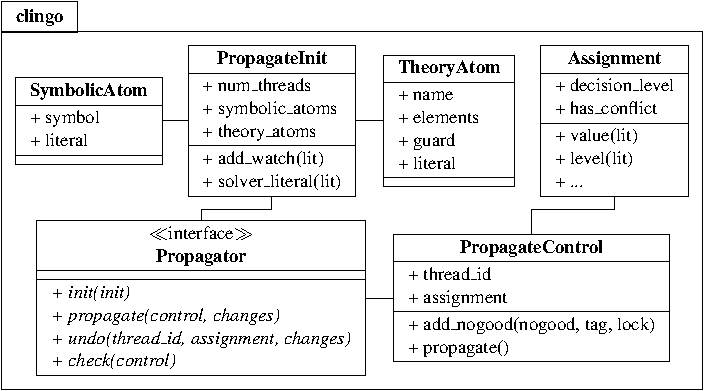
\includegraphics[width=\textwidth]{figures/python-interface}
  \caption{Class diagram of \clingo's (theory) propagator interface\label{fig:interface}}
\end{figure}
%
% To begin with,
The interface \code{Propagator} has to be implemented by each custom propagator.
After registering such a propagator with \clingo,
its functions are called during initialization and search as indicated % in the algorithm
in Figure~\ref{fig:cdcl}.
%
Function \code{Propagator.init}%
\footnote{For brevity, we below drop the qualification \code{Propagator} and use its function names unqualified.}
is called once before solving (Line~(\ref{fig:cdcl:init}) in Figure~\ref{fig:cdcl})
to allow for initializing data structures used during theory propagation.
It is invoked with a \code{PropagateInit} object providing access to symbolic (\code{SymbolicAtom}) as well as theory (\code{TheoryAtom}) atoms.
Both kinds of atoms are associated with program literals,\footnote{Program literals are also used in the \aspif\ format (see~\ref{sec:aspif}).} % ~\cite{gekakaosscwa16b}
which are in turn associated with solver literals.%
\footnote{Note that \clasp's preprocessor might associate a positive or even negative solver literal with multiple atoms.}
Program as well as solver literals are identified by non-zero integers, where positive and negative numbers represent positive or  negative literals, respectively.
In order to get notified about assignment changes, a propagator can set up watches on solver literals during initialization.

During search, function \codeClass{Propagator}{propagate} is called with a \code{PropagateControl} object
and a (non-empty) list of watched literals that got assigned in the recent round of unit propagation (Line~(\ref{fig:cdcl:propagate}) in Figure~\ref{fig:cdcl}).
The \code{PropagateControl} object can be used to inspect the current assignment, record nogoods, and trigger unit propagation.
Furthermore, to support multi-threaded solving,
its \code{thread\_id} property identifies the currently active thread,
each of which can be viewed as an independent instance of the CDCL algorithm in Figure~\ref{fig:cdcl}.%
%Hence, thread-specific state has to be associated with the \code{thread\_id}.
\footnote{%
Depending on the configuration of \clasp, threads can communicate with each other.
For example, some of the recorded nogoods can be shared.
This is transparent from the perspective of theory propagators.}
%
Function \codeClass{Propagator}{undo} is the counterpart of \codeClass{Propagator}{propagate}
and called whenever the solver retracts assignments to watched literals (Line~(\ref{fig:cdcl:undo}) in Figure~\ref{fig:cdcl}).
In addition to the list of watched literals that have been retracted (in chronological order),
it receives the identifier and the assignment of the active thread.
%
Finally, function \codeClass{Propagator}{check} is similar to \codeClass{Propagator}{propagate},
yet invoked without a list of changes.
Instead, it is (only) called on total assignments
(Line~(\ref{fig:cdcl:check}) in Figure~\ref{fig:cdcl}), independently of watches.
%
Overriding the empty default implementations of propagator methods is optional.
% Implementing the propagator methods, which default to empty implementations, is optional. % that does nothing.
For brevity, we below focus on implementations of the methods in \python,
while \lua\ or \C\ could be used as well.

For illustration,
consider Listing~\ref{prg:pigeon:propagator} giving a propagator for (half of) the pigeon-hole problem.
%
\lstinputlisting[linerange={1-10,12-39},float=t,mathescape=true,escapeinside={\#(}{\#)},basicstyle={\ttfamily\small},label={prg:pigeon:propagator},caption={Propagator for the pigeon-hole problem},language=clingo]{example/pigeon-py.lp}
%
Although this setting is constructed, it showcases central aspects
that are also relevant when implementing more complex propagators,
e.g., the \code{Pigeonator} is both stateful and can be used with multiple threads.
%
The underlying ASP encoding is given in Line~\ref{prg:pigeon:prop:rule1}:
A (choice) rule generates solution candidates by placing each of the $p$ pigeons in exactly one among $h$ holes.
While the rule commented out in Line~\ref{prg:pigeon:prop:rule2} would ensure that there is at most one pigeon per hole,
this constraint is handled by the \code{Pigeonator} class
implementing the \code{Propagator} interface (except for \code{check}) in Lines~\ref{prg:pigeon:prop:begin-init}--\ref{prg:pigeon:prop:end-undo}.
Whenever two pigeons are placed in the same hole, it adds a binary nogood forbidding the placement.
To this end,
it maintains data structures for, given a newly placed pigeon,
detecting whether there is a conflict.
%
More precisely, the propagator has two data members:
The \code{self.place} dictionary in Line~\ref{prg:pigeon:prop:member-place} maps solver literals
for \code{place}$/2$ atoms to their corresponding holes,
and the \code{self.state} list in Line~\ref{prg:pigeon:prop:member-state} stores for each solver thread its current placement of pigeons
as a mapping from holes to true solver literals for \code{place}$/2$ atoms.

Function \codeClass{Pigeonator}{init} in Lines~\ref{prg:pigeon:prop:begin-init}--\ref{prg:pigeon:prop:end-init}
sets up watches as well as the dictionaries in \code{self.place} and \code{self.state}.
%
To this end,
it traverses (symbolic) atoms over \code{place}$/2$ in Lines~\ref{prg:pigeon:prop:init:loop-atoms}--\ref{prg:pigeon:prop:init:end-loop-atoms}.
Each such atom is associated with a solver literal, % in \clasp,
obtained in Line~\ref{prg:pigeon:prop:init:map-literal}.
The mapping from the solver literal to its corresponding hole is then stored in the \code{self.place} dictionary in
Line~\ref{prg:pigeon:prop:init:map-lit-hole}.
%
In the last line of the loop, a watch is added for each solver literal at hand,
so that the solver calls \code{propagate} whenever a pigeon is placed. % in the hole as specified by the placement atom.
%
Finally, in Line~\ref{prg:pigeon:prop:init:state}, the \code{self.state} list
of placements per thread,
subject to change upon propagation and backjumping,
% Given a solving thread $i$, each state \code{self.state[$i$]} is a dictionary mapping holes to placement atoms given by their literals.
is initialized with empty dictionaries.

Function \codeClass{Pigeonator}{propagate}, given in Lines~\ref{prg:pigeon:prop:begin-prop}--\ref{prg:pigeon:prop:end-prop},
accesses \code{control.thread\_id} in Line~\ref{prg:pigeon:prop:prop:state}
to obtain the \code{holes} dictionary storing the active thread's current placement of pigeons.
% At first, in Line~\ref{prg:pigeon:prop:prop:state},
% \code{control.thread\_id} is used to obtain the dictionary storing the current thread's partial placement of pigeons.
The loop in Lines~\ref{prg:pigeon:prop:prop:begin-loop}--\ref{prg:pigeon:prop:prop:end-loop} then iterates over the list of changes,
i.e., solver literals representing newly placed pigeons.
After in Line~\ref{prg:pigeon:prop:prop:pigeon-to-hole}
determining the \code{hole} associated with a recently assigned literal,
% , the target \code{hole} associated with the current literal is obtained.
% Then,
\python's \code{setdefault} function is used to update the state:
Depending on whether \code{hole} already appears as a key in the \code{holes} dictionary,
the function either retrieves its associated literal or inserts the new literal under key \code{hole}. % into the dictionary.
While the latter case amounts to updating the placement of pigeons, the former signals a conflict,
triggered by recording a binary nogood in Line~\ref{prg:pigeon:prop:prop:add-clause}.
% In case of a conflict, the propagator adds a binary nogood in Line~\ref{prg:pigeon:prop:prop:add-clause} preventing such an invalid placement of pigeons.
Given that the solver has to resolve the conflict and backjump,
the call to \code{add\_nogood} always yields false, so that
propagation stops without processing remaining changes any further.\footnote{%
  The optional arguments \code{tag} and \code{lock} of \code{add\_nogood} can be used to control the scope and lifetime of recorded nogoods.
  Furthermore, in a propagator that does not add violated nogoods only, % but also unit-resulting nogoods
  function \code{control.propagate} can be invoked to trigger unit propagation.
  }
% Furthermore, using dictionaries \code{state[i]} and \code{place}, conflicts are detected in constant time.

Function \codeClass{Pigeonator}{undo} in Lines~\ref{prg:pigeon:prop:begin-undo}--\ref{prg:pigeon:prop:end-undo} resets a thread's placement of pigeons upon backjumping.
Similar to \codeClass{Pigeonator}{propagate}, % it is called by each solving thread.
the active thread's current placement
is obtained in Line~\ref{prg:pigeon:prop:undo:state},
and changes are traversed in Lines~\ref{prg:pigeon:prop:undo:begin-loop}--\ref{prg:pigeon:prop:undo:del}.
% The function then loops over the set of changes,
% that is, the literals corresponding to pigeons to be removed from the partial placement in Line~\ref{prg:pigeon:prop:undo:del}.
The latter correspond to retracted solver literals,
for which the condition in Line~\ref{prg:pigeon:prop:undo:test} makes sure
that exactly those stored in Line~\ref{prg:pigeon:prop:prop:setdefault} before are cleared,
thus reflecting that the \code{hole} determined in Line~\ref{prg:pigeon:prop:undo:pigeon-to-hole}
is free again.
%%
Finally,
function \code{main} in Lines~\ref{prg:pigeon:prop:begin-main}--\ref{prg:pigeon:prop:end-main} first registers the \code{Pigeonator} propagator in Line~\ref{prg:pigeon:prop:register},
and then initiates grounding and solving with \clingo.

%%% Local Variables:
%%% mode: latex
%%% TeX-master: "paper"
%%% End:

\section{Experiments}\label{sec:experiments}
%
\begin{table}[t]
\caption{Comparison of approximation techniques by 
(a) runtime and timeouts,
(b) diversification quality, and
(c) minimum distance}
\small
\parbox{.32\linewidth}{\centering
\begin{tabular}{|l||r|r|}

\hline
Class & \textit{T} & \textit{TO}  \\ 
\hline
\Alabel{3} & \textbf{165} & \textbf{70} \\
\Alabel{3}-\textit{true} & 200 & 113 \\ 
\Alabel{3}-\textit{all} & 202 & 118 \\ 
\Alabel{3}-\textit{rd} & 277 & 280 \\ 
\Alabel{3}-\textit{pg} & 317 & 351\\
\Alabel{3}-\textit{pg-l-rd} & 354 & 442\\
\Alabel{3}-\textit{false} & 351 & 443 \\ 
\Alabel{3}-\textit{pg-l} & 351 & 443\\
\Alabel{2}-\textit{true} & 482 & 618\\
\Alabel{2}-\textit{rd} & 474 & 648\\
\Alabel{1} & 482 & 672\\
\Alabel{2}-\textit{dist-to} & 528 & 689\\
\Alabel{2}-\textit{all} & 515 & 696\\
\Alabel{2}-\textit{false} & 532 & 696\\
\Alabel{2}-\textit{pg} & 542 & 708\\
\Alabel{2}-\textit{dist} & 572 & 773\\
\hline
\end{tabular} 
}
\parbox{.32\linewidth}{\centering
\begin{tabular}{|l||r|r|}

\hline
Class & \textit{S} & \textit{avg}\\ 
\hline
\Alabel{1} & \textbf{15} & 0.13\\
\Alabel{2}-\textit{dist-to} & 14 & 0.14\\ 
\Alabel{2}-\textit{pg} & 13 & \textbf{0.18}\\ 
\Alabel{3}-\textit{pg-l} & 11 & 0.17\\
\Alabel{3}-\textit{pg-l-rd} & 10 & 0.16\\
\Alabel{2}-\textit{all}  & 10 & 0.15\\
\Alabel{2}-\textit{dist} & 8 & 0.07\\ 
\Alabel{2}-\textit{false} & 8 & 0.15\\ 
\Alabel{2}-\textit{true} & 7 & 0.12\\ 
\Alabel{3}-\textit{false} & 6 & 0.16\\ 
\Alabel{2}-\textit{rd} & 5 & 0.12\\ 
\Alabel{3}-\textit{all}  & 5 & 0.08 \\ 
\Alabel{3}-\textit{true} & 4 & 0.08 \\ 
\Alabel{3}-\textit{rd} & 2 & 0.09 \\ 
\Alabel{3}-\textit{pg} & 1 & 0.09\\
%\Alabel{3}-Hdyn & 1 & 0.09\\ 
\Alabel{3} & 0 & 0.06\\

\hline
\end{tabular} 
}
\parbox{.32\linewidth}{\centering
\begin{tabular}{|l||r|r|}

\hline
Class & \textit{S} & \textit{avg}\\ 
\hline
\Alabel{1} & \textbf{15} & 12.25\\
\Alabel{2}-\textit{dist-to} & 13 & 10.38\\
\Alabel{3}-\textit{pg-l-rd } & 13 & 11.82 \\
\Alabel{2}-\textit{dist} & 12 & 5.31\\
\Alabel{3}-\textit{pg-l} & 12 & 11.10\\
\Alabel{2}-\textit{pg} & 10 & \textbf{12.86}\\
\Alabel{2}-\textit{rd} & 9 & 8.77 \\
\Alabel{3}-\textit{all}  & 7 & 3.99 \\ 
\Alabel{3}-\textit{true} & 6 & 4.00 \\ 
\Alabel{3}-\textit{false} & 6 & 7.07 \\ 
\Alabel{2}-\textit{false} & 6 & 6.80\\
\Alabel{2}-\textit{all}  & 4 & 6.98\\
\Alabel{2}-\textit{true} & 3 & 5.31\\
\Alabel{3}-\textit{rd} & 2 & 6.43\\
\Alabel{3} & 2 & 4.28\\
%\Alabel{3}-Hdyn & 1 & 2.90\\ 
\Alabel{3}-\textit{pg} & 0 & 2.79\\
\hline
\end{tabular} 
}
\label{tab:time_comparison_small}
\label{tab:diverse_comparison_small}
\label{tab:min_dist_comparison_small}
\end{table}
%
In this section, we present experiments focusing on the \emph{approximation} techniques of the \asprin\ system for obtaining most dissimilar optimal
solutions. 
%
While \emph{enumeration} and \emph{replication} provide exact results, they need to calculate and store a possibly exponential number of optimal
models or deal with a large search space, respectively.
%
Those techniques are therefore not effective for most practical applications.
%
For Algorithm~\Alabel{2}, we considered the variations \textit{rd}, \textit{pg}, \textit{true}, \textit{false}, and \textit{all} .
%
In \textit{dist}, we issued no timeout for the computation of the partial interpretation, 
while in \textit{dist-to}, we set a timeout for this computation of half the total possible runtime.
%
For Algorithm~\Alabel{3}, we consider the variations that include no extra ASP computation, namely, 
\textit{rd}, \textit{pg}, \textit{true}, \textit{false}, and \textit{all} .
%
We also evaluated a version without any heuristic modification (named simply \Alabel{3}).
%
Furthermore, following \cite{nadel11a}, 
we considered a variation of \textit{pg}, viz.~\textit{pg-l}, 
where the atoms of the selected partial interpretation are given a higher priority, 
and \textit{pg-l-rd}, extending \textit{pg-l} by fixing initially a random sign to all atoms not appearing in the partial interpretation.

We gathered 186 instances from six different classes: \emph{Design Space exploration (DSE)} from~\cite{angeglharesc13a}, \emph{Timetabling (CTT)}
from~\cite{basotainsc13a}, \emph{Crossing minimization} from the ASP competition 2013, \emph{Metabolic network expansion} from \cite{schthi09a},
\emph{Biological network repair} from \cite{geguivscsithve10a} and \emph{Circuit Diagnosis} from~\cite{sidiqqi11a}.
Since we required instances with multiple optimal solutions, we exclusively focused on Pareto optimality. 
DSE and CTT are inherently multi-objective and therefore we could naturally define a Pareto preference for them. 
For the other classes, we turned single-objective into multi-objective optimization problems by distributing their optimization statements.
First, we split the atoms in the optimization statements into four or eight groups evenly. 
We chose for each group the same preference type, either cardinality or subset minimization, and aggregated them by means of Pareto preference.
We calculated optimal solutions regarding these Pareto preferences.
The same was done for CTT and DSE.
An instance was selected if for some Pareto preference ten optimal solutions could be obtained within 600 seconds by \asprin. 
This method generated 816 instances in total. 
We ran the benchmarks on a cluster of Linux machines with dual Xeon E5520 quad-core 2.26 GHz processors and 48 GB RAM. 
We restricted the runtime to 600 seconds and the memory usage to 20 GB RAM.

Since algorithms~\Alabel{1} and \Alabel{2} involve querying programs over preferences, 
we started by evaluating the different query techniques. 
%
For that, we executed \Alabel{1} with query methods \Qlabel{1} to \Qlabel{4} on all selected instances,
stopping after the first $\mathit{solveQuery}$ call was finished.
%
%We achieved that by first calculating an optimal solution and then finding another optimal solution fulfilling the query that the model has to be dissimilar.
The performance of query techniques \Qlabel{2}, \Qlabel{3}, and \Qlabel{4} was similar regarding runtime and only \Qlabel{1} was clearly worse.
We selected \Qlabel{4} for the remaining experiments due to its slightly lower runtime. 
For more detailed tables, we refer to~\cite{roscwa16b}. % \ref{sec:suptables}.

Next, we approximated four most diverse optimal models with methods \Alabel{1} to \Alabel{3}. 
%
We measured runtime and two quality measures.
The first, called diversification quality~\cite{nadel11a},
gives the sum of the Hamming distances among all pairs of solutions normalized to values between zero and one.
The second is the minimum distance among all pairs of solutions of a set in percent.
%
The solution set size of four was chosen because~\cite{shimazu01a} 
claims that three solutions is the optimal amount for a user,
and considering one additional solution provides further insight into the different quality measures. 
%
For all algorithms that do not use heuristics for diversification, 
we instead enabled heuristics preferring a negative sign for the atoms appearing in preference statements. 
This was observed in~\cite{brderosc15b} to improve performance.

Table~\ref{tab:time_comparison_small}(a) provides in column \textit{T} the average runtime and in column \textit{TO} the sum of timeouts. 
The different methods are ordered by the number of timeouts. 
The best results in a column are shown in bold. 
We see that \Alabel{3} is by far the fastest with 70 timeouts, solving 91\% of the instances. 
Heuristic variations of \Alabel{3} perform the best after that. 
Less invasive heuristics achieve similar runtimes with 113-118 timeouts.
More sophisticated heuristics perform worse at 349-443 timeouts.
In a range from 618 to 773 timeouts, non-heuristic methods solve the least instances by a significant margin.
The results are in tune with the nature of the methods. 
Heuristics modifying the solving process for diversity decrease the performance 
in comparison with solving heuristics aimed at performance, 
but not as much as more complex methods involving preferences over optimal models. 

In particular, non-heuristic methods show many timeouts. 
If we tried to analyze the quality of the solutions by assuming worst possible values for the instances that timed out,
the results would be dominated by these instances. 
To avoid that, we calculated a score independent of the runtime.
We considered all possible parings of the different methods. 
For each pair, we compared only instances where both found a solution set.
The method with better quality value for the majority of instances receives a point. 
Finally, we ordered the subsequent tables according to that score. 
 
In Table~\ref{tab:diverse_comparison_small}(b), for each method we see the score in column \textit{S}, and 
the average of the diversification quality (over the instances solved by the method) in column \textit{avg}. 
This way, we can examine the quality a method has achieved compared to other methods, and also the individual average quality.
\Alabel{1} has the best quality with a score of 15, followed by \Alabel{2}-\textit{dist-to}, \Alabel{2}-\textit{pg}, \Alabel{3}-\textit{pg-l} and \Alabel{3}-\textit{pg-l-rd}.
All of those techniques regard the whole previous solution set to calculate the next solution
and guide the solving strictly to diversity.
\Alabel{2}-\textit{pg}, \Alabel{3}-\textit{pg-l} and \Alabel{3}-\textit{pg-l-rd } are also the first, second and third place, respectively, for average diversification quality. 
Next, with scores ranging from 10-7, we see \Alabel{2} methods 
that do not take into account the whole previous set, 
or that were simply unable to find many solutions at all, as in the case of \Alabel{2}-\textit{dist}. 
Finally, we observe that \Alabel{3} variations only regarding the last solution or no previous information 
perform worst in score and average. 
In these cases, the heuristic does not seem to be strong enough to steer the solving to high quality solution sets, 
and \Alabel{3} uses no heuristic or optimization techniques to ensure diverse solutions.

In analogy to Table~\ref{tab:diverse_comparison_small}(b),
Table~\ref{tab:min_dist_comparison_small}(c) provides information for the minimum distance among the solutions. 
%
% The overall grouping of the methods is similar to Table~\ref{tab:diverse_comparison_small}(b). 
%
The best methods considering score and average minimum distance, 
viz.\ \Alabel{1}, \Alabel{2}-\textit{dist-to}, \Alabel{3}-\textit{pg-l-rd}, \Alabel{3}-\textit{pg-l}, \Alabel{2}-\textit{pg}, utilize information from the whole
previous solution set and have strict diversification techniques. 
%\comment{I cut the part about the different behavior of min distance and diversification. The data is not that clear and it saves space. Maybe if we have space left in the end...}

Overall, plain heuristic methods perform better in regards to runtime 
while more complex methods, depending on all previous solutions, lead to better quality. 
%
Furthermore, \Alabel{3}-\textit{pg-l-rd } and \Alabel{3}-\textit{pg-l} provide the best trade-off between performance and quality. 
%
While \Alabel{1}, \Alabel{2}-\textit{dist-to} and \Alabel{2}-\textit{pg} achieve higher quality, they could solve only 18\%, 16\% and 13\% of the instances. 
%
On the other hand, \Alabel{3}-\textit{pg-l-rd } and \Alabel{3}-\textit{pg-l} provide good diversification quality and minimum distance while solving 46\% of the instances. 
%
%\comment{this section is enough for general conclusion: plain heuristic: fast but bad, maxmin: slow but good, more complex heuristic: tradeoff}


%%% Local Variables: 
%%% mode: latex
%%% TeX-master: "paper"
%%% End: 


\section{Discussion}\label{sec:discussion}

Various ways of adding domain-specific information have been explored in the literature.
%
A prominent approach is to implement forms of preferential reasoning
% , like reasoning wrt inclusion-minimal models, 
by directing choices through
a given partial order on literals~\cite{cacacale96a,rogima10a,giumar12a}.
%
To some degree, this can be simulated by heuristic modifiers like
\hpre{a}{\texttt{false}}{1}
that allow for computing a (single) inclusion-minimal model.
However, as detailed in \cite{rogima10a}, enumerating all such models needs additional constraints
or downstream tester programs.
Similarly,
\cite{balduccini11b} modifies the heuristic of the ASP solver \textit{smodels} to accommodate learning from smaller instances.
See also~\cite{falepf01a,falemari07a}.
Most notably,
\cite{rintanen12a} achieves impressive results in planning by equipping a SAT solver with
planning-specific heuristics.
%
All aforementioned approaches need customized changes to solver implementations.
%
Hence, it will be interesting to investigate how these approaches can be expressed and combined in
our declarative framework.
%
Declarative approaches to incorporating control knowledge can be found in heuristic planning.
For instance, \cite{backab00a} harness temporal logic formulas, while \cite{sierra04a} also uses
dedicated predicates for controlling backtracking in a forward planner.
%
However,
care must be taken when it comes to modifying a solver's heuristics.
Although it may lead to great improvements, it may just as well lead to a degradation of search.
In fact, the restriction of choice variables may result in exponentially larger search spaces~\cite{jajuni05a}.
This issue is reflected in our choice of heuristic modifiers, 
ranging from an \texttt{init}ial bias,
over a continued yet scalable one by \texttt{factor},
to a strict preference with \texttt{level}.

To sum up,
we introduced a declarative framework for incorporating domain-specific heuristics into ASP solving.
The seamless integration into ASP's input language provides us with a general and flexible tool for
expressing domain-specific heuristics.
As such, we believe it to be the first of its kind.
Our heuristic framework offers completely new possibilities of applying, experimenting, and studying
domain-specific heuristics in a uniform setting.
Our example heuristics merely provide first indications on the prospect of our approach,
but much more systematic empirical studies are needed to exploit its full power.


%%% Local Variables: 
%%% mode: latex
%%% TeX-master: "paper"
%%% End: 

\bibliography{paper} % {lit,akku,procs}

\end{document}

%%% Local Variables:
%%% mode: latex
%%% TeX-master: t
%%% End:
